% Version  Date        Author            Notes
% 1        ?           Tobias Lutz
% 2        April 2016  Tasnad Kernetzky  Updated to new IEEEtran class (v. 1.8)
%
%
\documentclass[journal, a4paper]{IEEEtran}

% check if we are running lua(la)tex and load font related packages appropriately
\usepackage{ifluatex}
\ifluatex
    \usepackage{fontspec}
\else
    \usepackage[T1]{fontenc}
    \usepackage[utf8]{inputenc}
\fi

% some very useful LaTeX packages include:
%\usepackage{cite}      % Written by Donald Arseneau
                        % V1.6 and later of IEEEtran pre-defines the format
                        % of the cite.sty package \cite{} output to follow
                        % that of IEEE. Loading the cite package will
                        % result in citation numbers being automatically
                        % sorted and properly "ranged". i.e.,
                        % [1], [9], [2], [7], [5], [6]
                        % (without using cite.sty)
                        % will become:
                        % [1], [2], [5]--[7], [9] (using cite.sty)
                        % cite.sty's \cite will automatically add leading
                        % space, if needed. Use cite.sty's noadjust option
                        % (cite.sty V3.8 and later) if you want to turn this
                        % off. cite.sty is already installed on most LaTeX
                        % systems. The latest version can be obtained at:
                        % http://www.ctan.org/tex-archive/macros/latex/contrib/supported/cite/

\usepackage{graphicx}   % Written by David Carlisle and Sebastian Rahtz
                        % Required if you want graphics, photos, etc.
                        % graphicx.sty is already installed on most LaTeX
                        % systems. The latest version and documentation can
                        % be obtained at:
                        % http://www.ctan.org/tex-archive/macros/latex/required/graphics/
                        % Another good source of documentation is "Using
                        % Imported Graphics in LaTeX2e" by Keith Reckdahl
                        % which can be found as esplatex.ps and epslatex.pdf
                        % at: http://www.ctan.org/tex-archive/info/

%\usepackage{psfrag}    % Written by Craig Barratt, Michael C. Grant,
                        % and David Carlisle
                        % This package allows you to substitute LaTeX
                        % commands for text in imported EPS graphic files.
                        % In this way, LaTeX symbols can be placed into
                        % graphics that have been generated by other
                        % applications. You must use latex->dvips->ps2pdf
                        % workflow (not direct pdf output from pdflatex) if
                        % you wish to use this capability because it works
                        % via some PostScript tricks. Alternatively, the
                        % graphics could be processed as separate files via
                        % psfrag and dvips, then converted to PDF for
                        % inclusion in the main file which uses pdflatex.
                        % Docs are in "The PSfrag System" by Michael C. Grant
                        % and David Carlisle. There is also some information
                        % about using psfrag in "Using Imported Graphics in
                        % LaTeX2e" by Keith Reckdahl which documents the
                        % graphicx package (see above). The psfrag package
                        % and documentation can be obtained at:
                        % http://www.ctan.org/tex-archive/macros/latex/contrib/supported/psfrag/

%\usepackage{subfigure} % Written by Steven Douglas Cochran
                        % This package makes it easy to put subfigures
                        % in your figures. i.e., "figure 1a and 1b"
                        % Docs are in "Using Imported Graphics in LaTeX2e"
                        % by Keith Reckdahl which also documents the graphicx
                        % package (see above). subfigure.sty is already
                        % installed on most LaTeX systems. The latest version
                        % and documentation can be obtained at:
                        % http://www.ctan.org/tex-archive/macros/latex/contrib/supported/subfigure/

%\usepackage{url}       % Written by Donald Arseneau
                        % Provides better support for handling and breaking
                        % URLs. url.sty is already installed on most LaTeX
                        % systems. The latest version can be obtained at:
                        % http://www.ctan.org/tex-archive/macros/latex/contrib/other/misc/
                        % Read the url.sty source comments for usage information.

%\usepackage{stfloats}  % Written by Sigitas Tolusis
                        % Gives LaTeX2e the ability to do double column
                        % floats at the bottom of the page as well as the top.
                        % (e.g., "\begin{figure*}[!b]" is not normally
                        % possible in LaTeX2e). This is an invasive package
                        % which rewrites many portions of the LaTeX2e output
                        % routines. It may not work with other packages that
                        % modify the LaTeX2e output routine and/or with other
                        % versions of LaTeX. The latest version and
                        % documentation can be obtained at:
                        % http://www.ctan.org/tex-archive/macros/latex/contrib/supported/sttools/
                        % Documentation is contained in the stfloats.sty
                        % comments as well as in the presfull.pdf file.
                        % Do not use the stfloats baselinefloat ability as
                        % IEEE does not allow \baselineskip to stretch.
                        % Authors submitting work to the IEEE should note
                        % that IEEE rarely uses double column equations and
                        % that authors should try to avoid such use.
                        % Do not be tempted to use the cuted.sty or
                        % midfloat.sty package (by the same author) as IEEE
                        % does not format its papers in such ways.

%\usepackage{amsmath}   % From the American Mathematical Society
                        % A popular package that provides many helpful commands
                        % for dealing with mathematics. Note that the AMSmath
                        % package sets \interdisplaylinepenalty to 10000 thus
                        % preventing page breaks from occurring within multiline
                        % equations. Use:
%\interdisplaylinepenalty=2500
                        % after loading amsmath to restore such page breaks
                        % as IEEEtran.cls normally does. amsmath.sty is already
                        % installed on most LaTeX systems. The latest version
                        % and documentation can be obtained at:
                        % http://www.ctan.org/tex-archive/macros/latex/required/amslatex/math/



% Other popular packages for formatting tables and equations include:

%\usepackage{array}
% Frank Mittelbach's and David Carlisle's array.sty which improves the
% LaTeX2e array and tabular environments to provide better appearances and
% additional user controls. array.sty is already installed on most systems.
% The latest version and documentation can be obtained at:
% http://www.ctan.org/tex-archive/macros/latex/required/tools/

% V1.6 of IEEEtran contains the IEEEeqnarray family of commands that can
% be used to generate multiline equations as well as matrices, tables, etc.

% Also of notable interest:
% Scott Pakin's eqparbox package for creating (automatically sized) equal
% width boxes. Available:
% http://www.ctan.org/tex-archive/macros/latex/contrib/supported/eqparbox/

% *** Do not adjust lengths that control margins, column widths, etc. ***
% *** Do not use packages that alter fonts (such as pslatex).         ***
% There should be no need to do such things with IEEEtran.cls V1.6 and later.


% Your document starts here!
\begin{document}

% Define document title and author
\title{Guidelines for Writing a Seminar Report}
\author{Firstname Lastname
\thanks{Advisor: Firstname~Lastname,~M.Sc., Lehrstuhl für Nachrichtentechnik, TUM, WS 2017/2018.}}
\markboth{Hauptseminar Digitale Kommunikationssysteme}{}
\maketitle

% Write abstract here
\begin{abstract}
The short abstract (50-80 words) is intended to give the reader an overview of the work.
Keep in mind that he does not known the work yet.
\end{abstract}

% Each section begins with a \section{title} command
\section{Introduction}
% \IEEEPARstart{}{} creates a tall first letter for this first paragraph
\IEEEPARstart{T}{his} section introduces the topic and leads the reader on to the main part.
Do not forget to mention the papers your seminar work is based on!

% Main Part
\section{Main Part}
% LaTeX takes complete care of your document layout ...
The presentation's content is summarized in the report in 4~pages.
% ... but you can insert a line break manually with two backslashes, if needed: \\
The author should fill, but not exceed, this space. \\
The report should be a self-contained report, so that it can be understood without studying additional literature.

\section{Format}
The report can be written in \LaTeX{} or Microsoft Word, but \LaTeX{} is definitely preferred.
Its appearance should be as close to this document as possible to achieve consistency in the proceedings.

% You can cite a book or paper by using \cite{reference}.
% The references will be defined at the end of this .tex file in the bibliography
References should be cited as numbers, and should be ordered by their appearance (example: ``... as shown in \cite{HOP96}, ...'').
Only references that are actually cited can be listed in the references section.
The references' format should be evident from the examples in this text.

References should be of academic character and should be published and accessible.
Your advisor can answer your questions regarding literature research.
You must cite all used sources.
Examples of good references include text books and scientific journals or conference proceedings.
If possible, citing internet pages should be avoided. In particular, Wikipedia is \emph{not} an appropriate reference in academic reports.
Avoiding references in languages other than English is recommended.

% You can reference tables and figure by using the \ref{label} command. Each table and figure needs to have a UNIQUE label.
Figures and tables should be labeled and numbered, such as in Table~\ref{tab:simParameters} and Fig.~\ref{fig:tf_plot}.

% This is how you define a table: the [!hbt] means that LaTeX is forced (by the !) to place the table exactly here (by h), or if that doesnt work because of a pagebreak or so, it tries to place the table to the bottom of the page (by b) or the top (by t).
\begin{table}[!hbt]
    % Center the table
    \begin{center}
    % Title of the table
    \caption{Simulation Parameters}
    \label{tab:simParameters}
    % Table itself: here we have two columns which are centered and have lines to the left, right and in the middle: |c|c|
    \begin{tabular}{|c|c|}
        % To create a horizontal line, type \hline
        \hline
        % To end a column type &
        % For a linebreak type \\
        Information message length & $k=16000$ bit \\
        \hline
        Radio segment size & $b=160$ bit \\
        \hline
        Rate of component codes & $R_{cc}=1/3$\\
        \hline
        Polynomial of component encoders & $[1 , 33/37 , 25/37]_8$\\
        \hline
    \end{tabular}
    \end{center}
\end{table}

% If you have questions about how to write mathematical formulas in LaTeX, please read a LaTeX book or the 'Not So Short Introduction to LaTeX': tobi.oetiker.ch/lshort/lshort.pdf

% This is how you include a eps figure in your document. LaTeX only accepts EPS or TIFF files.
\begin{figure}[!hbt]
    % Center the figure.
    \begin{center}
    % Include the eps file, scale it such that it's width equals the column width. You can also put width=8cm for example...
    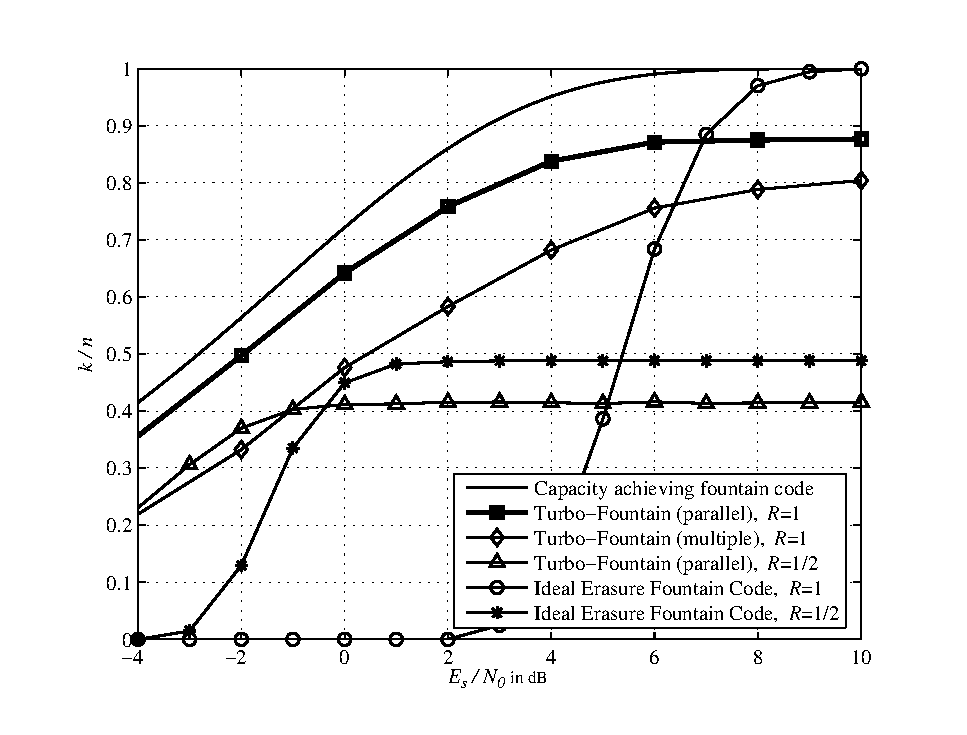
\includegraphics[width=\columnwidth]{figs/plot_tf.eps}
    % Create a subtitle for the figure.
    \caption{Simulation results on the AWGN channel. Average throughput $k/n$ vs $E_s/N_0$.}
    % Define the label of the figure. It's good to use 'fig:title', so you know that the label belongs to a figure.
    \label{fig:tf_plot}
    \end{center}
\end{figure}

\section{Filling this page}
Gallia est omnis divisa in partes tres, quarum unam incolunt Belgae, aliam Aquitani, tertiam qui ipsorum lingua Celtae, nostra Galli appellantur. Hi omnes lingua, institutis, legibus inter se differunt. Gallos ab Aquitanis Garumna flumen, a Belgis Matrona et Sequana dividit. Horum omnium fortissimi sunt Belgae, propterea quod a cultu atque humanitate provinciae longissime absunt, minimeque ad eos mercatores saepe commeant atque ea quae ad effeminandos animos pertinent important, proximique sunt Germanis, qui trans Rhenum incolunt, quibuscum continenter bellum gerunt.

\section{Conclusion}
This section summarizes the paper. Now the reader knows your work, you can go into detail a little bit more about the main aspects.


% Now we need a bibliography:
\begin{thebibliography}{1}

    %Each item starts with a \bibitem{reference} command and the details thereafter.
    \bibitem{HOP96} % Transaction paper
    J.~Hagenauer, E.~Offer, and L.~Papke. Iterative decoding of binary block
    and convolutional codes. {\em IEEE Trans. Inform. Theory},
    vol.~42, no.~2, pp.~429–-445, Mar. 1996.

    \bibitem{MJH06} % Conference paper
    T.~Mayer, H.~Jenkac, and J.~Hagenauer. Turbo base-station cooperation for intercell interference cancellation. {\em IEEE Int. Conf. Commun. (ICC)}, Istanbul, Turkey, pp.~356--361, June 2006.

    \bibitem{Proakis} % Book
    J.~G.~Proakis. {\em Digital Communications}. McGraw-Hill Book Co.,
    New York, USA, 3rd edition, 1995.

    \bibitem{talk} % Web document
    P.~N.~Edwards. How to give a talk: Changing the culture of academic public speaking.
    http://www.si.umich.edu/~pne/acadtalk.htm.

    \bibitem{5}
    IEEE Transactions \LaTeX{} and Microsoft Word Style Files.
    http://www.ieee.org/web/publications/authors/transjnl/index.html

\end{thebibliography}

% Your document ends here!
\end{document}
